%% IDE has R L T A 3
%% timetable has L R A 3
\documentclass[12pt,a4paper,twoside]{article}
\usepackage{graphicx,fancyhdr}
\pdfpagebox=4

\setlength{\parindent}{0cm}
\setlength{\parskip}{2ex plus1ex minus 0.5ex}

\addtolength{\evensidemargin}{-2.5cm}
\addtolength{\oddsidemargin}{-0.5cm}
\addtolength{\textwidth}{3cm}

\addtolength{\headheight}{0.2cm}
\addtolength{\topmargin}{-2.5cm}
\addtolength{\textheight}{2.5cm}

% \newcommand{\source}[1]{\textbf{\verb^#1^}}}
\renewcommand{\_}{\texttt{\symbol{95}}}
\addtolength{\fboxsep}{0.1cm}
\newcommand{\param}[1]{\textit{\textrm{\textmd{#1}}}}
\newcommand{\codebar}{\rule{\textwidth}{0.3mm}}
\newcommand{\todo}{\textbf{TODO}}

\newlength{\codelen}
\newcommand{\code}[1]
{\begin{center}\fbox{\parbox{16cm}{\texttt{#1}}}\end{center}}

\newcommand{\mission}[1]{\item[#1:]}
% \newcommand{\mission}[1]{\texttt{#1}\hspace{3mm}}

\fancyhead{}
\fancyhead[RO,LE]{\thepage}
\fancyhead[LO,RE]{ROBOC Summer School Exercises}
\fancyfoot{}
\pagestyle{fancy}
% \pagestyle{empty}

\setcounter{secnumdepth}{1}

\newenvironment{bulletlist}
{
	\begin{itemize}
	\addtolength{\itemsep}{-1mm}
	% \setlength{\itemsep}{0ex}
	\setlength{\parsep}{0ex}
}
{
	\end{itemize}
}

\newenvironment{alphalist}
{
	\begin{enumerate}
	\setlength{\itemsep}{0ex}
	\setlength{\parsep}{0ex}
	\renewcommand{\labelenumi}{(\alph{enumi})}
}
{
	\end{enumerate}
}

\newenvironment{numericlist}
{
	\begin{enumerate}
	\addtolength{\itemsep}{-1mm}
	% \setlength{\itemsep}{0ex}
	\setlength{\parsep}{0ex}
}
{
	\end{enumerate}
}

\usepackage{hyperref}
\begin{document}

\centerline{\textbf{\LARGE ROBOC Summer School Exercises}}
\vspace{0.5cm}
\centerline{August 2011}
\centerline{Author: David Ingram}
\centerline{2010 Revision: David Eyers (\texttt{David.Eyers@cl.cam.ac.uk})}
\centerline{2011 Revision: Ian Davies (\texttt{Ian.Davies@cl.cam.ac.uk})}

{ \parskip 1mm plus 1pt \tableofcontents }

%\section*{Variables}
%
%\textit{Variables} in programming are different from in Maths:
%\begin{bulletlist}
%\item In maths, variables are unknown quantities
%\item In programming, variables refer to numbers which can change
%\item The equals (\verb^=^) sign means \textit{assignment}
%\item You can call your variables anything: x, y, pos, distance, banana etc
%\end{bulletlist}
%
%\section*{Loops}
%
%Loops are a way to repeat the same set of actions multiple times.
%
%\begin{verbatim}
%total = 0
%loop n from 1 to 10
%   total = total + n
%end
%\end{verbatim}
%
%The counter variable (\verb^n^ in this loop)
%keeps track of how many times it has repeated.
%\verb^loop^ blocks are terminated by the \verb^end^ keyword.
%The actions to be repeated are all those between the \verb^loop^
%and the \verb^end^.

%\newpage
\section{Logo Mode} \label{sec:logo-mode}

\subsection{Example programs}

\subsubsection*{Polygon}

\begin{verbatim}
polygon(6, 100)

fn polygon(edges, size)
   angle = 360 / edges
   loop i from 0 to edges - 1
      move size
      turn angle
   end
end
\end{verbatim}

\subsubsection*{Waterwheel}

\begin{verbatim}
turn -90
waterwheel(12, 75)

fn waterwheel(edges, size)
   angle = 360 / edges
   decoration = size / 2
   loop i from 1 to edges
      move size
      square(decoration)
      turn angle
   end
end

fn square(side)
   loop i from 1 to 4
      move side
      turn -90
   end
end
\end{verbatim}

\subsubsection*{Spiral}

\begin{verbatim}
spiral(0)

fn spiral(size)
   if size > 300
      return
   end
   move size
   turn 90
   spiral(size + 2)
end
\end{verbatim}

\subsubsection*{Fractal---von Koch Snowflake curve}

\begin{verbatim}
origin(Left)
segment(600, 6)

fn segment(scale, detail)
   if detail = 0
      move scale
   else
      segment(scale / 3, detail - 1)
      turn -60
      segment(scale / 3, detail - 1)
      turn 120
      segment(scale / 3, detail - 1)
      turn -60
      segment(scale / 3, detail - 1)
   end
end
\end{verbatim}

\begin{figure}[t]
\centering
%\fbox{
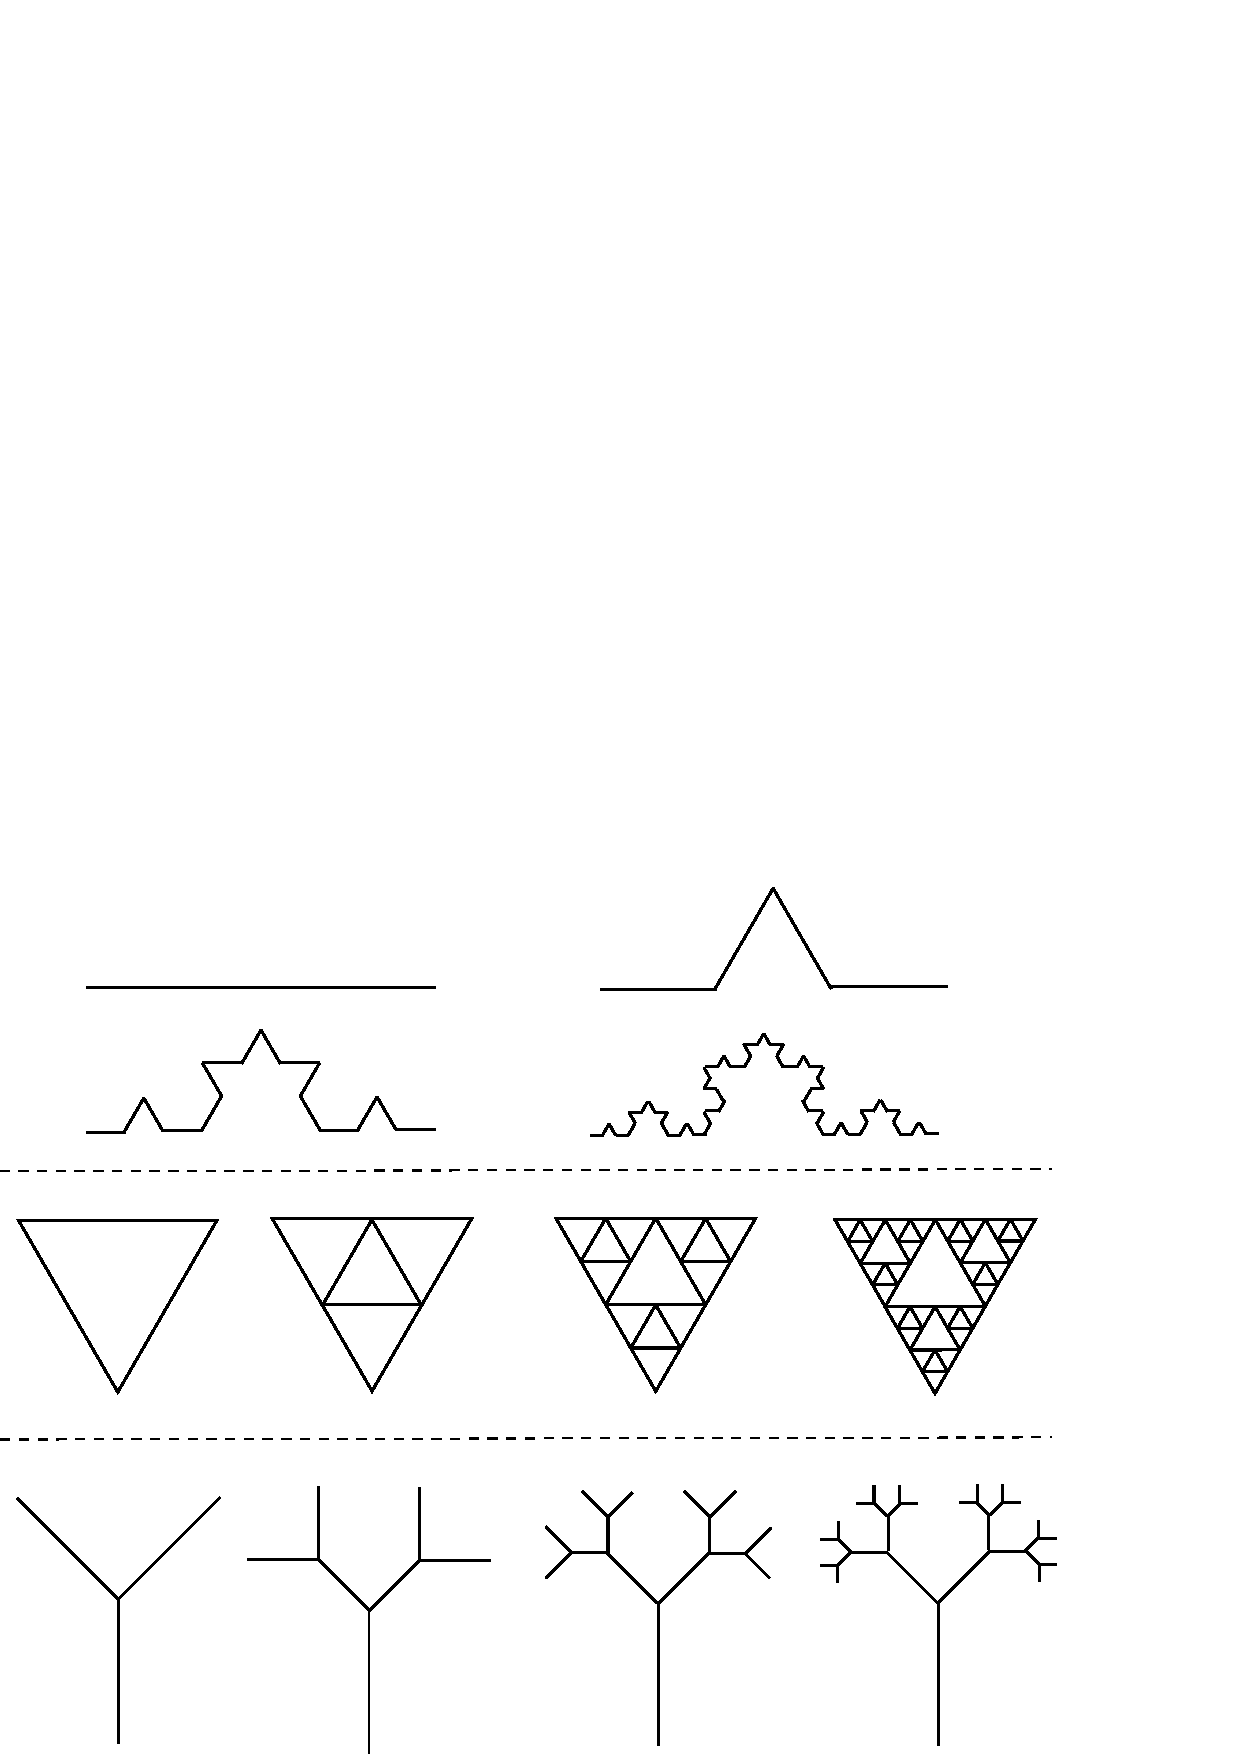
\includegraphics[scale=0.5,trim=10mm 10mm 10mm 155mm]{diagrams/new_fractal}
%}
\caption{Levels of detail for snowflake, triangle and tree fractals}
\label{fractal}
\end{figure}
\subsection{Exercises}

\begin{numericlist}
\item Run the spiral square program.
	Change the angle from 90 to 91 degrees and test what difference
	this makes.
\item Run the polygon program, then modify it to draw a circle.
\item Run the waterwheel program. Change it to make the paddles on the
	waterwheel triangular.
\item Write a program to draw a chessboard.
\item Run the fractal snowflake program. Try changing the detail parameter of the segment function. Then follow the instructions in the Triangles program to create the triangle fractal shown in the middle row of Figure \ref{fractal}. 
\item (extension) Write a similar program to draw a fractal tree, as shown in the last row of Figure \ref{fractal}.
%
      \item (extension) Try creating a library of functions that allow
        you to form words on the canvas (probably just pick a few
        letters from the alphabet!). Your letters will be joined by a
        line when the turtle moves from one letter to the next. You
        could try positioning this line so that the whole word looks
        like it is underlined.
%
\end{numericlist}


%\newpage
\section{Robot Mode}\label{sec:robot-mode}

\subsection{A very primitive robot}

\begin{verbatim}
loop
   if touch() = Wall
      turn 2
   end
   move
end
\end{verbatim}

\textit{How can we improve this, so it doesn't keep going back and forth?}

\subsection{Some ideas}

\begin{bulletlist}
\item Use \verb^leftside^ or \verb^rightside^ to spot fruit or turn
	into a side passage
\item To turn alternately left or right, create a variable called \verb^dir^
	(for example) and change it from \verb^-1^ to \verb^1^ each time you turn:
	\begin{verbatim}
	dir = 1
	...
	turn dir
	dir = -dir
	\end{verbatim}
\item Use senses to work out when you are in a dead end and then turn around
\item Spin around on the spot checking for fruit ahead with \verb^look^
\item Use a counter variable to take an action every \verb^k^ steps
\item Keep track of the distance travelled or the direction you are
	facing in, and use this to change the robot's behaviour
\end{bulletlist}

\subsection{Hints for missions}

\begin{description}
\mission{SEARCH}
	Avoid a pre-planned route---use sensors instead to alert the robot to
	nearby targets. If you can hit ten targets your robot passes
	this mission. Expert programmers might be able to find thirty or more!

\mission{CHESS}
	The grid pattern is fixed and regular, so this time you don't need to
	use sensors to tell you where to go.
	Instead you will need to plan your route carefully to trace over the
	lines, and write loops to avoid repeating steps in your program.

\mission{TRAIL}
	Use sensors and turn towards the footprints to make sure
	your robot stays on course.

\mission{CLEANUP}
	You need to use sensors to detect the edges of the pool.
	This is quite difficult to get right.

\mission{MAZE}
	This type of maze can be solved by
	following either the left or right wall.

%\mission{REFUEL}

\mission{MINE}
	Efficiency is key---you will only pass this test if you
	waste no time gathering items almost continuously throughout the
	time allowed.

%\mission{PALACE}

\mission{FIELD}
	Try to avoid walking in straight lines for long distances, when
	there may be flowers nearby.

\mission{TREASURE}
	The gems are found in clusters. Once you have found a
	gem, look around nearby for the rest of the cluster, then
	go exploring for the next set.

\mission{VINE}
	This challenge requires recursion and backtracking.

%\mission{RAID}
\end{description}

%\newpage
\section{Art Mode}\label{sec:art-mode}

\subsection{Example programs}

\subsubsection*{Shapes}

\begin{verbatim}
ink(Blue)
spot(100, 200, 50)
circle(300, 200, 50)
box(450, 150, 100, 100)
\end{verbatim}

\subsubsection*{Vector}

\begin{verbatim}
ink(Red)
line(100, 400, 400, 400)
line(400, 400, 250, 100)
line(250, 100, 100, 400)
\end{verbatim}

\subsubsection*{Images}

\begin{verbatim}
x = 60
y = 150
width = 20
height = 8

loop i from 1 to width
   loop j from 1 to height
      if i % 4 = 0
         icon(x + i * 30, y + j * 30, YellowFlower)
      else
         icon(x + i * 30, y + j * 30, Clover)
      end
   end
end
\end{verbatim}

\subsubsection*{Triangle}

\begin{verbatim}
size = 10

loop y from 1 to size
   loop x from 1 to y
      icon(50 + x * 30, 100 + y * 30, Clover)
   end
end
\end{verbatim}

\subsubsection*{Stars}

\begin{verbatim}
star(300, 300, Sky, 100, 200)
star(600, 400, Purple, 200, 200)
star(450, 200, Orange, 125, 200)

fn star(x, y, colour, size, spines)
   ink(colour)
   angle = 0
   loop i from 1 to spines
      x0 = x + (size * cos(angle))
      y0 = y + (size * sin(angle))
      line(x, y, x0, y0)
      angle = angle + (2 * Pi / spines)
   end
end
\end{verbatim}

\subsubsection*{Sketch}

\begin{verbatim}
listen(MouseDrag + MouseClick)
loop
   input()
   if eventclass = MouseDrag
      line(lastx, lasty, mousex, mousey)
   else
      plot(mousex, mousey)
   end
   lastx = mousex
   lasty = mousey
end
\end{verbatim}

\subsubsection*{Lander}

\begin{verbatim}
var CursorLeft = 128, CursorRight = 129
var CursorUp = 130, CursorDown = 131

var x = 100, y = 500, vx = 0, vy = 0, ax = 0, ay = 0
var t, lastt, pause = 20000, power = 3/20

draw_world()

lastt = time()
listen(KeyPress + KeyRelease)
loop
   if poll() > 0
      if eventclass = KeyPress
         if keyval = CursorLeft
            ax = -power
         elif keyval = CursorRight
            ax = power
         elif keyval = CursorUp
            ay = -power
         elif keyval = CursorDown
            ay = power
         end
      else
         if keyval = CursorLeft or keyval = CursorRight
            ax = 0
         elif keyval = CursorUp or keyval = CursorDown
            ay = 0
         end
      end
   end

   ink(White)
   box(x - 10, y - 10, 20, 20)

   vx = vx + ax
   vy = vy + ay
   x = x + vx
   y = y + vy
   ink(Red)
   box(x - 10, y - 10, 20, 20)
   
   t = time()
   if t - lastt < pause
      delay(pause - (t - lastt))
   end
   lastt = time()
end
\end{verbatim}

\subsection{Exercises}

\begin{numericlist}
\item Run the shapes program. Now make the spot a bit smaller, put the spot
		inside the circle and put the square under the circle.
\item Run the vector program, then change the red triangle into a green square.
		Next def{i}ne and test your own function to draw rectangles.
\item Run the images program, then change the flower stripes to be horizontal
		instead of vertical. Next, make the stripes diagonal.
\item Run the triangle program, then change it to display the following
		instead:\\
\begin{center}
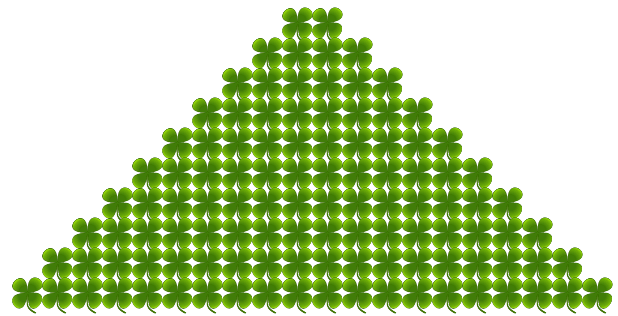
\includegraphics[scale=0.35,angle=0]{screenshots/artpixel/triangle2}
\end{center}
\item Run the stars program, then adapt it to draw ellipses instead.
\item Test the sketch program, and change it so that the right mouse
		button draws in a different colour.
\item Control the lander program with the cursor keys, and try to drive
		the red square around the course without destroying any of the walls.
		Then add gravity to the program, and horizontal friction.
\end{numericlist}

%\newpage
\section{3D Mode}


Consult ``3D mode'' section in the reference manual for description of the environment.

\subsection{Example programs}

\subsubsection*{Transformations}

\begin{verbatim}
translate(30, 0, 0)
rotatey(20)
scale(5, 1, 2)
cube()
\end{verbatim}

This is best understood by building up from the the basic cube
one transformation at a time.
Consider what goes wrong if the rotation comes after the scaling
or before the translation...?

\subsubsection*{Stonehenge arch}

\begin{verbatim}
translate(0, 0, -1)
mark()
   scale(6, 2, 1)
   cube()
recall()
translate(-2, 0, -1.5)
mark()
   scale(1, 1, 4)
   cube()
recall()
translate(4, 0, 0)
mark()
   scale(1, 1, 4)
   cube()
recall()
\end{verbatim}

\subsubsection*{Robot}

\begin{verbatim}
translate(0, 0, -4)
mark()
   rotatey(90)
   scale(2, 2, 2)
   cylinder()
recall()
translate(0, 0, 3.5)
mark()
   scale(2, 1, 6)
   cube()
recall()
mark()
   rotatey(45)
   translate(0, 0, 2)
   mark()
      scale(1, 1, 4)
      cube()
   recall()
   translate(0, 0, 2)
   pyramid()
recall()
mark()
   rotatey(-45)
   translate(0, 0, 2)
   scale(1, 1, 4)
   cube()
recall()
translate(0, 0, 2)
mark()
   scale(0.5, 0.5, 4)
   cylinder()
recall()
translate(0, 0, 3)
scale(2, 2, 2)
sphere()
\end{verbatim}

\subsubsection*{Steps}

\begin{minipage}{8cm}
\begin{verbatim}
translate(0,0,-4)
loop i from 1 to 10
   translate(1, 0, 0.5)
   mark()
      scale(1, 8, 1)
      if i = 6
         colour(Red)
      end
      cube()
   recall()
end
\end{verbatim}
\end{minipage}
\begin{minipage}{8cm}
	\begin{center}
	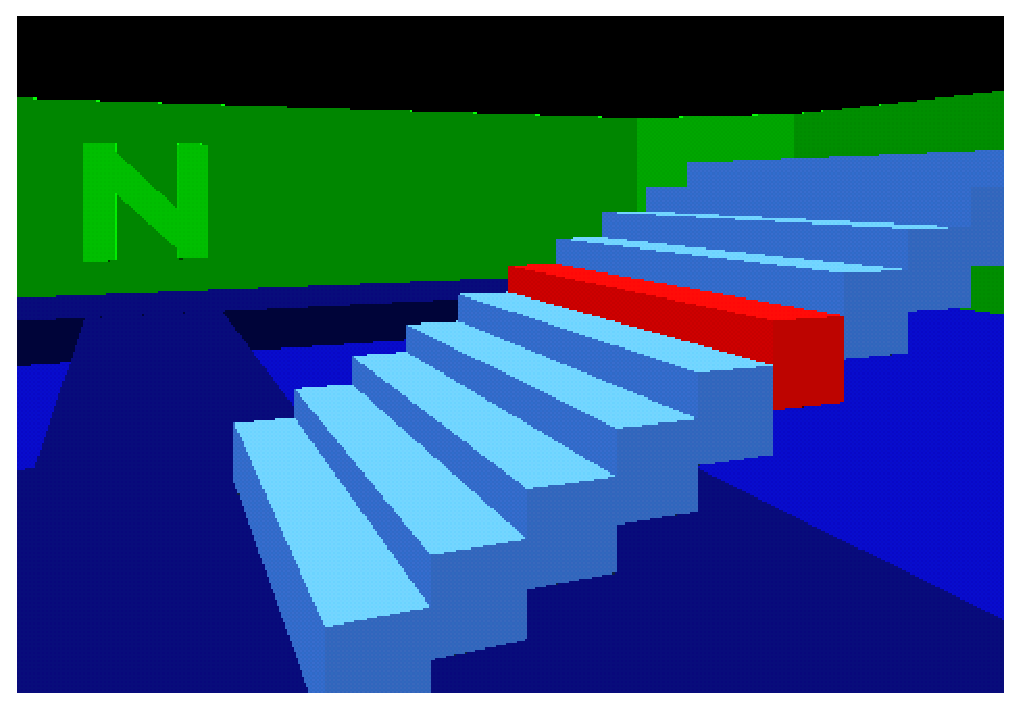
\includegraphics[scale=0.5,angle=0]{screenshots/3d/steps}
	\end{center}
\end{minipage}

\subsubsection*{Wheel}

\begin{minipage}{8cm}
\begin{verbatim}
scale(3,3,3)
torus(0.1)
loop i from 1 to 4
   mark()
      scale(0.05, 0.05, 1)
      cylinder()
   recall()
   rotatey(45)
end
\end{verbatim}
\end{minipage}
\begin{minipage}{8cm}
	\begin{center}
	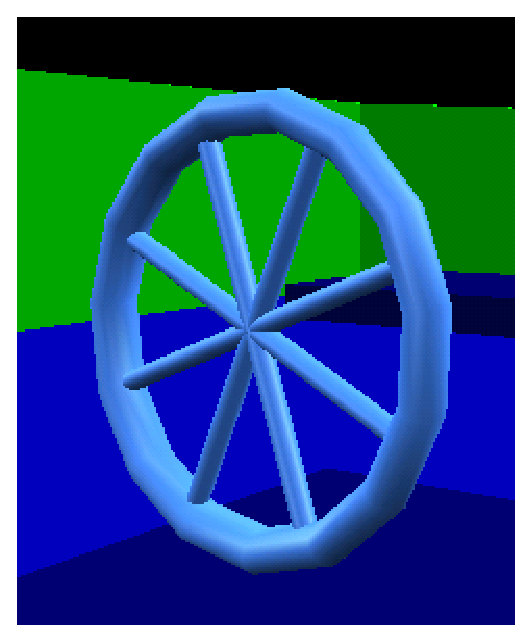
\includegraphics[scale=0.6,angle=0]{screenshots/3d/wheel}
	\end{center}
\end{minipage}

\subsection{Short assignments}

\begin{numericlist}
\item Build a tree (see picture for an example). It should be
      green, with a brown trunk and a grey pot underneath.\\
		\begin{center}
      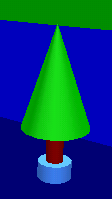
\includegraphics[scale=0.75,angle=0]{screenshots/3d/tree}\hspace{1cm}
      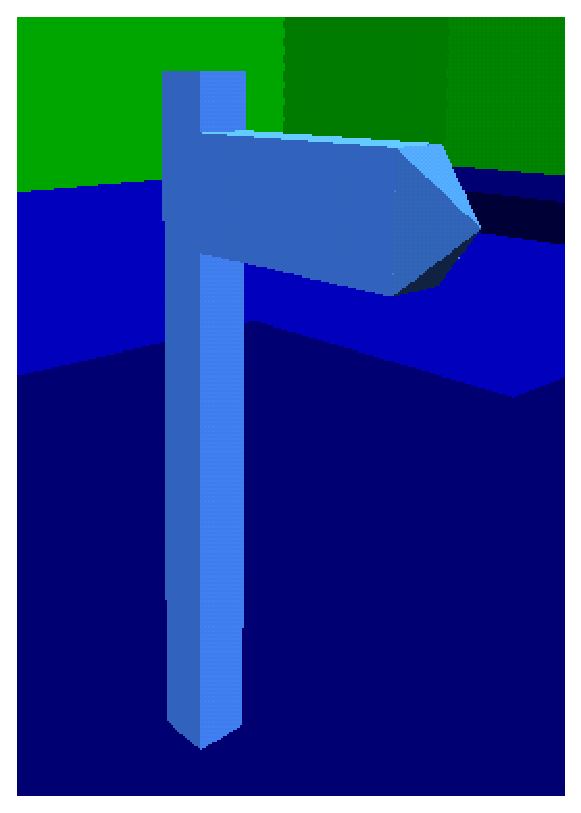
\includegraphics[scale=0.4,angle=0]{screenshots/3d/signpost}
		\end{center}
\item Make an avenue of 10 trees, using a loop.
\item Build a signpost. The pointed end is made from a pyramid.
\item Modify the stonehenge arch program to create a circle of
      arches, using a loop.\\
		\begin{center}
      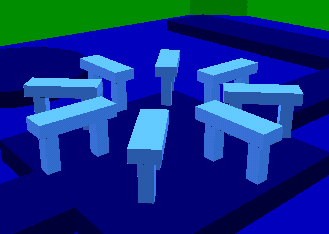
\includegraphics[scale=0.5,angle=0]{screenshots/3d/stone_circle}
		\end{center}
\end{numericlist}

\subsection{Long assignments}

\begin{numericlist}

\item Construct a plane, like the one shown. Notice that the
      cockpit is made from a sphere and the engines are
		cylinders. Which shapes is the tail made from?\\
		\begin{center}
		
\includegraphics[scale=0.6,angle=0]{screenshots/3d/plane1}
		
\includegraphics[scale=0.6,angle=0]{screenshots/3d/plane2}
		\end{center}
\item Build a castle. It should have 4 round towers, 4 walls,
      a raised drawbridge and a square keep with a flag on top.

\end{numericlist}

%\newpage
\section{Extension: Text Mode}\label{sec:text-mode}

\subsection{Example programs}

\subsubsection*{Table of squares}

\begin{verbatim}
loop i from 1 to 25
   print i : "squared =" : square(i) ; ", sqrt =" : sqrt(i)
end

fn square(x)
   answer = x * x
   return answer
end
\end{verbatim}

\subsubsection*{Calculate factorials recursively}

\begin{verbatim}
a = 6
print "Factorial of" : a : "is:" : fact(a)

fn fact(n)
   if n = 1
      return 1
   end
   return n * fact(n - 1)
end
\end{verbatim}

\subsubsection*{Factorisation}

\begin{verbatim}
factorise(100)

fn factorise(n)
   loop i from 2 to sqrt(n)
      if n % i = 0
         print i
         factorise(n / i)
         return
      end
   end
   print n
end
\end{verbatim}

\subsubsection*{Units conversion}

\begin{verbatim}
loop c from 0 to 35
   print c : "degrees C =" : convert(c) : "degrees F"
end

fn convert(c)
   return (c * 9 / 5) + 32
end
\end{verbatim}

\subsubsection*{Selection sort}

\begin{verbatim}
n = 100
var a[n]

loop i from 0 to n - 1
   a[i] = random(1, 1000)
end

print "First ten of" : n : "items (unsorted):"
display()

selection()

print "First ten of" : n : "items (sorted):"
display()

fn selection()
   loop i from 0 to n - 2
      min = i
      loop j from i + 1 to n - 1
         if a[j] < a[min]
            min = j
         end
      end
      swap(i, min)
   end
end

fn swap(i, j)
   temp = a[i]
   a[i] = a[j]
   a[j] = temp
end

fn display()
   loop i from 0 to 9
      print "Array item" : i : "is" : a[i]
   end
end
\end{verbatim}

\subsubsection*{Throwing dice}

\begin{verbatim}
n = 60

loop i from 1 to n
   x = random(1, 6)
   print i : " " : x
end
\end{verbatim}

\subsection{Exercises}

\begin{numericlist}
\item Run the table of squares and factorial programs.
	Make a new program which prints a table of factorials.
\item Time how long the selection sort program takes to run on
	different sizes of array.
\item Run the dice program.
	Extend this to keep track of how many of each number are thrown
	using an array, such as \texttt{var count[6]}, and report the
	final counts at the end.
	Investigate averages with more throws.
	Change it to a two dice experiment.
\item Run the units conversion program.
	Investigate whether there is a temperature which is the same in
	both units.
	Then change the program so that it offers a menu, with four options:
	to convert celsius to fahrenheit, fahrenheit to celsius, inches to
	centimetres or centimetres to inches. Use the \texttt{read()}
	function to get a response from the user, and to input the value
	to be converted. A response of \texttt{exit} could be used to return
	to the menu.
\end{numericlist}

%\newpage
\section{Extension: Networking}\label{sec:networking}

\subsection{Example programs}

\subsubsection*{Text chat}

\begin{verbatim}
listen(NetEvent)
self("alice")

loop
   if poll() ~ 0
      print message
   else
      text = read()
      print text
      send("bob", text)
   end
end
\end{verbatim}

\subsection{Exercises}

\begin{numericlist}
\item Pair up with somebody else, and test the text chat program.
	You will need to modify the \texttt{self} and \texttt{send}
	commands to direct messages to your partner.
\end{numericlist}

\end{document}
